% !TeX program = xelatex
% The Nordling Lab Presentation example implemented using Beamer by Jose Chang and Torbjörn Nordling.
% Copyright 2018 by Nordling Lab
%
% You are hereby granted the permission to freely copy and modify this file as you see fit, as long as
% you acknowledges Nordling Lab.
%
% NOTE You need to use XeLaTeX to compile this file!

% Use these lines for a 16:9 aspect ratio no scaling version in the presentation
\documentclass[aspectratio=169]{beamer}
\mode<presentation>{
    \usetheme{NordlingLab169}
}

% Load packages
\usepackage[english]{babel}
\let\latinencoding\relax
\usepackage{xltxtra} %Needed to use Candara font
\setsansfont{Candara}

\usepackage{graphicx} %Needed to insert images
\usepackage[absolute,overlay]{textpos}
\graphicspath{{../../result/multi_model_results/pdf/}{../../result/focused_results/pdf/}{../../result_nofeature/experiments_zeroshot_Dallen vs Gary/static/comparison_results/pdf/}{Figures/}{../../feature_selection/fs_results_v2/png/}}
\usepackage[yyyymmdd]{datetime} %Needed to get date on ISO format
\renewcommand{\dateseparator}{--}

\usepackage{listings, lstautogobble}
\usepackage{verbatim}
\usepackage[sort&compress,square,comma,authoryear]{natbib}
\usepackage{subcaption}
\usepackage{tikz,lipsum,lmodern}
\usetikzlibrary{positioning,arrows.meta}
\usepackage[most]{tcolorbox}
\usepackage{fancyvrb}
\usepackage{array}
\usepackage{caption}
\captionsetup[figure]{font=tiny,labelfont=tiny}

\usepackage{changepage}
\usepackage{ragged2e}

\usepackage{booktabs}
\setcitestyle{round}
\bibliographystyle{apalike}

\usepackage{multicol}
\usepackage{multirow}
\usepackage{hyperref}
\usepackage{xcolor}
\usepackage{colortbl}

\lstdefinestyle{DOS}
{
    backgroundcolor=\color[gray]{0.9},
    basicstyle=\scriptsize\color{black}\ttfamily
}

\lstset{
    autogobble=true
}

\newenvironment{metaverbatim}{\verbatim}{\endverbatim}

\title[Benchmarking LLMs for FT]{Benchmarking LLMs with Pre-Extracted Features for MDS-UPDRS Finger Tapping Assessment}
\author[Gary Wang]{Gary Wang}
\institute[NCKU]{Nordling Lab @
    Dept. of Mechanical Engineering\\
    National Cheng Kung University
        No. 1 University rd., Tainan 70101, Taiwan}
\date{\today}

% Table of contents at each section
\AtBeginSection[]{
    \begin{frame}<beamer>{Outline}
        \tableofcontents[currentsection]
    \end{frame}
}


%%%%%%%%%%%%%%%%%%%%%%%%%%%%%%%%%%%%%%%%%%%%%%%%%%%%%
\begin{document}

\setbeamertemplate{background}[NLTitle]
\setbeamertemplate{footline}[NLTitle]
\begin{frame}
    \titlepage
\end{frame}

\setbeamertemplate{background}[NLCC]
\setbeamertemplate{footline}[NLCC]
\begin{frame}<beamer>{Outline}
    \tableofcontents[sectionstyle=show,subsectionstyle=show/shaded/hide]
\end{frame}

%%%%%%%%%%%%%%%%%%%%%%%%%%%%%%%%%%%%%%%%%%%%%%%%%%%%%
\section{Background}

\begin{frame}
    \frametitle{Background}
    \begin{itemize}
    \item Parkinson's Disease (PD)
    \begin{itemize}
        \item Neurological disorder affecting 11.8 million globally in 2021.
        \item Characterized by bradykinesia (slow decremental movement).
    \end{itemize}
    \item MDS-UPDRS Item 3.4: Finger Tapping (FT)
    \begin{itemize}
        \item A rating scale (0--4) for diagnosing bradykinesia severity.
        \item Assesses interruptions, slowing, and amplitude decrement.
    \end{itemize}
    \item Previous Work
    \begin{itemize}
        \item Single-model evaluation (ChatGPT-4) showed potential with few-shot prompting.
        \item Best result: 61.1\% accuracy, 0.39 MAE, inter-rater ICC(3,k) = 0.85.
    \end{itemize}
    \item This Study
    \begin{itemize}
        \item Benchmark \textbf{14 LLM configurations} across multiple model families.
        \item Compare zero-shot vs.\ few-shot prompting strategies.
        \item Evaluate using MAE, RMSE, Correlation, Weighted Kappa, and Wasserstein Distance.
    \end{itemize}
    \end{itemize}
\end{frame}


\begin{frame}
    \frametitle{Models Under Evaluation}
    \begin{itemize}
        \item \textbf{Gemini 3 Flash} (Google)
        \begin{itemize}
            \item Few-shot and zero-shot configurations
        \end{itemize}
        \item \textbf{DeepSeek-R1} (DeepSeek)
        \begin{itemize}
            \item 32B few-shot \& zero-shot, 70B few-shot \& zero-shot
        \end{itemize}
        \item \textbf{Qwen 2.5} (Alibaba)
        \begin{itemize}
            \item 7B few-shot \& zero-shot, 32B few-shot \& zero-shot, 72B few-shot \& zero-shot
        \end{itemize}
        \item \textbf{Qwen3} (Alibaba)
        \begin{itemize}
            \item 30B few-shot \& zero-shot
        \end{itemize}
    \end{itemize}
    \vspace{0.5em}
    Each session scored \textbf{10 times} independently to capture model variability.
\end{frame}


%%%%%%%%%%%%%%%%%%%%%%%%%%%%%%%%%%%%%%%%%%%%%%%%%%%%%
\section{Methods}

\begin{frame}
    \frametitle{Prompt Design: This Study vs.\ Previous Work (Dallen 2024)}
    {\color{black}{\scriptsize
    \begin{table}
        \centering
        \setlength{\tabcolsep}{4pt}
        \begin{tabular}{lcc}
        \toprule
        \textbf{Prompt Element} & \textbf{Dallen 2024 (Prompt D)} & \textbf{This Study} \\
        \midrule
        Task description        & \checkmark & \checkmark \\
        MDS-UPDRS criteria      & \checkmark & \checkmark \\
        Raw trajectory CSV      & \checkmark\ (10-tap, 5 cols) & $\times$ \\
        Pre-extracted features  & $\times$ & \checkmark\ (8 features) \\
        Python analysis script  & \checkmark & $\times$ \\
        Few-shot examples       & \checkmark\ (TXT file, 4 scores) & \checkmark\ (embedded, 4 scores) \\
        \midrule
        \textbf{Approx.\ input tokens} & \textbf{$\sim$12,000--15,000} & \textbf{$\sim$633 (ZS) / $\sim$1,525 (FS)} \\
        \textbf{Token reduction}       & --                            & \textbf{$\sim$8--23$\times$ fewer} \\
        \midrule
        Models evaluated        & ChatGPT-4 only & 14 LLM configurations \\
        Best MAE                & 0.39 & 0.53 \\
        Best Kappa              & -- & 0.54 \\
        \bottomrule
        \end{tabular}
    \end{table}
    }}
    \vspace{0.3em}
    \tiny{ZS = zero-shot, FS = few-shot.}
\end{frame}

\begin{frame}
    \frametitle{Experimental Pipeline}
    \centering
    \begin{tikzpicture}[
        >=stealth,
        box/.style={draw=black!60, fill=blue!8, rounded corners=3pt,
                    minimum width=1.7cm, minimum height=0.55cm,
                    font=\tiny, align=center},
        proc/.style={draw=orange!80, fill=orange!15, rounded corners=3pt,
                    minimum width=1.7cm, minimum height=0.55cm,
                    font=\tiny\bfseries, align=center},
        arr/.style={->, thin, black!70},
        node distance=0.3cm and 0.35cm
    ]
    % Row 1: Data collection
    \node[box] (vid)  {Video\\Recording};
    \node[box, right=of vid]  (cot)  {CoTracker\\Tracking};
    \node[box, right=of cot]  (csv)  {Raw\\Trajectory CSV};
    \node[box, right=of csv]  (fext) {Feature\\Extraction};
    \node[box, right=of fext] (cand) {$\sim$50 Candidate\\Features};

    % Row 2: Feature selection (snake back)
    \node[proc, below=0.5cm of cand] (corr) {FS Pipeline\\(28 Methods,\\LOOCV)};
    \node[box, left=of corr]  (sel)  {8 Selected\\Features};
    \node[box, left=of sel]   (prom) {Prompt\\Construction\\(ZS / FS)};
    \node[box, left=of prom]  (llm)  {LLM Inference\\(14 configs\\$\times$ 10 runs)};
    \node[box, left=of llm]   (med)  {Median\\Score};

    % Row 3: Evaluation
    \node[proc, below=0.5cm of med]  (eval) {Evaluation\\Metrics};
    \node[box, right=of eval] (gt)   {Neurologist\\Consensus\\(2 raters)};

    % Arrows Row 1
    \draw[arr] (vid)  -- (cot);
    \draw[arr] (cot)  -- (csv);
    \draw[arr] (csv)  -- (fext);
    \draw[arr] (fext) -- (cand);
    \draw[arr] (cand) -- (corr);

    % Arrows Row 2 (snake)
    \draw[arr] (corr) -- (sel);
    \draw[arr] (sel)  -- (prom);
    \draw[arr] (prom) -- (llm);
    \draw[arr] (llm)  -- (med);
    \draw[arr] (med)  -- (eval);
    \draw[arr] (gt)   -- (eval);
    \end{tikzpicture}
    \vspace{0.3em}\\
    \tiny{Features selected by FS pipeline (28 methods, LOOCV, $n$=53). See next slides for details.}
\end{frame}

%%%%%%%%%%%%%%%%%%%%%%%%%%%%%%%%%%%%%%%%%%%%%%%%%%%%%
\begin{frame}
    \frametitle{Feature Selection Pipeline}
    \centering
    \scalebox{0.78}{%
    \begin{tikzpicture}[
        node distance=0.55cm,
        box/.style={rectangle, rounded corners, draw, thick,
                    minimum width=11cm, minimum height=0.9cm, align=center},
        arr/.style={-Stealth, thick},
    ]
        \node[box, fill=blue!10]   (s1) {\textbf{Stage 1:} Run \textbf{28 FS methods} (filter / embedded / wrapper) on 149 features};
        \node[box, fill=orange!10, below=of s1] (s2) {\textbf{Stage 2:} For each subset $\to$ \textbf{LOOCV} with fixed predictor (MLP-8, ReLU, Adam, $\alpha$=1.0)};
        \node[box, fill=green!10,  below=of s2] (s3) {\textbf{Stage 3:} Score with \textbf{4 metrics} (MAE, Spearman, Kappa, Adj.\ Acc.) + 2000-iter bootstrap CIs};
        \node[box, fill=red!10,    below=of s3] (s4) {\textbf{Stage 4:} Rank FS methods by \textbf{Composite} = mean of normalised metrics};
        \node[box, fill=purple!10, below=of s4] (s5) {\textbf{Stage 5:} Filter (Kappa $\ge0.5$, $N_\text{feat}<15$) $\to$ count \textbf{feature inclusion frequency} (17/28 pass)};
        \draw[arr] (s1) -- (s2);
        \draw[arr] (s2) -- (s3);
        \draw[arr] (s3) -- (s4);
        \draw[arr] (s4) -- (s5);
    \end{tikzpicture}}
\end{frame}

%%%%%%%%%%%%%%%%%%%%%%%%%%%%%%%%%%%%%%%%%%%%%%%%%%%%%
\begin{frame}
    \frametitle{Signal Preprocessing}
    \scriptsize
    \begin{columns}[T]
        \column{0.48\textwidth}
        \textbf{Raw input:} 2D coordinates of thumb \& index finger per frame.\\[0.4em]
        \begin{tabular}{p{2.2cm}p{4.6cm}}
            \texttt{Distance} & $\sqrt{(\Delta X)^2+(\Delta Y)^2}$ (px) \\[0.3em]
            \texttt{Norm\_Dist} & $\frac{\text{Distance}-\min(d)}{\max(d)-\min(d)} \in [0,1]$ \\[0.3em]
            \texttt{Speed}    & $d(\text{Distance})/dt$ \quad (px/s) \\[0.3em]
            \texttt{Speed\_norm}    & $d(\text{Norm\_Dist})/dt$ \\[0.3em]
            \texttt{Accel.}   & $d(\text{Speed})/dt$ \quad (px/s$^2$) \\[0.3em]
            \texttt{Accel.\_norm}   & $d(\text{Speed\_norm})/dt$ \\
        \end{tabular}\\[0.5em]
        \textbf{Peak} = frame of maximum finger separation (tap).\\
        \textbf{Valley} = frame of minimum separation between taps.

        \column{0.48\textwidth}
        \textbf{Per-tap amplitude:}\\
        $A_k = d(\text{peak}_k) - \tfrac{d(v_\text{before})+d(v_\text{after})}{2}$\\[0.3em]
        \textbf{Normalised amplitude:}\\
        $\tilde{A}_k = \dfrac{A_k}{d_\text{max} - d_\text{min}}$\\[0.1em]
        {\scriptsize removes hand-size \& camera-distance confounds}\\[0.4em]
        \textbf{Inter-tap interval (ITI):}\\
        $\text{ITI}_k = t(\text{peak}_{k+1}) - t(\text{peak}_k)$\\[0.4em]
        \textbf{Opening phase} of tap $k$: $\text{valley}_\text{before} \to \text{peak}_k$\\
        \textbf{Closing phase} of tap $k$: $\text{peak}_k \to \text{valley}_\text{after}$
    \end{columns}
\end{frame}

%%%%%%%%%%%%%%%%%%%%%%%%%%%%%%%%%%%%%%%%%%%%%%%%%%%%%
\begin{frame}
    \frametitle{Feature Groups Overview --- Unified Clinical Grouping (149)}
    \scriptsize\centering
    \begin{tabular}{llc}
        \toprule
        \textbf{Group} & \textbf{Clinical Domain} & \textbf{N} \\
        \midrule
        A.\ Kinematics      & Raw finger displacement range \& variability                & 48 \\
        B.\ Speed           & Tapping rate, opening/closing velocity, and their decrement & 35 \\
        C.\ Amplitude       & Finger-opening size, shape, and progressive decrement       & 31 \\
        D.\ Rhythm          & Temporal regularity of inter-tap intervals                  & 14 \\
        E.\ Freezing        & Movement pauses and halts                                   &  7 \\
        F.\ Task Completion & Ability to perform the full 10-tap sequence                 &  5 \\
        G.\ Phase Asymmetry & Timing asymmetry between opening and closing                &  9 \\
        \midrule
        \textbf{Total} & & \textbf{149} \\
        \bottomrule
    \end{tabular}\\[0.5em]
\end{frame}

%%%%%%%%%%%%%%%%%%%%%%%%%%%%%%%%%%%%%%%%%%%%%%%%%%%%%
\begin{frame}
    \frametitle{Group A: Kinematics (48)}
    \scriptsize
    \begin{columns}[T]
        \column{0.55\textwidth}
        \renewcommand{\arraystretch}{1.2}
        \begin{tabular}{p{4.2cm}p{2.8cm}}
            \toprule
            \textbf{Feature} & \textbf{Definition} \\
            \midrule
            \texttt{finger\_mvmnt\_thumb\_x\_*} (6) & $|\Delta X_\text{thumb}|$, 6 stats \\
            \texttt{finger\_mvmnt\_thumb\_y\_*} (6) & $|\Delta Y_\text{thumb}|$, 6 stats \\
            \texttt{finger\_mvmnt\_thumb\_dist\_*} (6) & $\sqrt{\Delta X_T^2+\Delta Y_T^2}$, 6 stats \\
            \texttt{finger\_mvmnt\_index\_x\_*} (6) & $|\Delta X_\text{index}|$, 6 stats \\
            \texttt{finger\_mvmnt\_index\_y\_*} (6) & $|\Delta Y_\text{index}|$, 6 stats \\
            \texttt{finger\_mvmnt\_index\_dist\_*} (6) & $\sqrt{\Delta X_I^2+\Delta Y_I^2}$, 6 stats \\
            \texttt{acceleration\_*} (6) & $|d^2(\text{Distance})/dt^2|$ (px/s$^2$), 6 stats \\
            \texttt{acceleration\_norm\_*} (6) & $|d^2(\text{Norm\_Dist})/dt^2|$, 6 stats \\
            \bottomrule
        \end{tabular}\\[0.3em]
        \emph{Stats: median, IQR, mean, min, max, std}

        \column{0.42\textwidth}
        \textbf{Motivation}\\[0.3em]
        PD patients exhibit reduced range of motion and increased spatial variability due to bradykinesia and rigidity.\\[0.4em]
        Thumb and index finger are tracked separately: thumb acts as the pivot; index executes the tap. Both contribute independent kinematic information.\\[0.4em]
        Normalised acceleration captures relative sharpness; raw acceleration (px/s$^2$) preserves absolute scale for cross-subject comparison.
    \end{columns}
\end{frame}

%%%%%%%%%%%%%%%%%%%%%%%%%%%%%%%%%%%%%%%%%%%%%%%%%%%%%
\begin{frame}
    \frametitle{Group B: Speed (35)}
    \scriptsize
    \begin{columns}[T]
        \column{0.58\textwidth}
        \renewcommand{\arraystretch}{1.2}
        \begin{tabular}{p{3.8cm}p{3.4cm}}
            \toprule
            \textbf{Feature} & \textbf{Definition} \\
            \midrule
            \texttt{speed\_*} (6) & $|d(\text{Distance})/dt|$ (px/s), 6 stats \\
            \texttt{speed\_norm\_*} (6) & $|d(\text{Norm\_Dist})/dt|$, 6 stats \\
            \texttt{frequency\_*} (6) & $f_k = 1/\text{ITI}_k$ (Hz), 6 stats \\
            \texttt{freq\_lr\_slope} & Slope of linear fit to $f_k$ \\
            \texttt{freq\_lr\_fitness\_r2} & $R^2$ of frequency--time fit \\
            \texttt{freq\_fit\_min\_degree} & Fixed $= 1$ (linear model) \\
            \texttt{V\_open\_*} (3) & $\max(\dot{d})$ opening (px/s), 3 stats \\
            \texttt{V\_open\_norm\_*} (3) & $\max(\dot{d})/(d_\text{max}{-}d_\text{min})$, 3 stats \\
            \texttt{V\_close\_*} (3) & $|\min(\dot{d})|$ closing (px/s), 3 stats \\
            \texttt{V\_close\_norm\_*} (3) & $|\min(\dot{d})|/(d_\text{max}{-}d_\text{min})$, 3 stats \\
            \texttt{R\_V\_open} & $\mathrm{med}(V[-3:])/\mathrm{med}(V[:3])$, opening \\
            \texttt{R\_V\_close} & Same ratio for closing \\
            \bottomrule
        \end{tabular}

        \column{0.39\textwidth}
        \textbf{Motivation}\\[0.3em]
        Tapping speed directly reflects bradykinesia. Progressive deceleration (\texttt{freq\_lr\_slope}$<$0) is a key MDS-UPDRS 3.4 sub-criterion.\\[0.4em]
        Normalised speed removes amplitude confound; raw speed (px/s) preserves absolute scale. \texttt{R\_V\_open/close} measure velocity decrement analogous to amplitude decrement.
    \end{columns}
\end{frame}

%%%%%%%%%%%%%%%%%%%%%%%%%%%%%%%%%%%%%%%%%%%%%%%%%%%%%
\begin{frame}
    \frametitle{Group C: Amplitude --- Statistics (1/2, total 31)}
    \scriptsize
    $A_k = d(\text{peak}_k) - \text{mean(adjacent valleys)}$\\[0.2em]
    \begin{columns}[T]
        \column{0.55\textwidth}
        \renewcommand{\arraystretch}{1.1}
        \begin{tabular}{p{4.2cm}p{2.8cm}}
            \toprule
            \textbf{Feature} & \textbf{Definition} \\
            \midrule
            \texttt{amplitude\_*} (6) & 6 stats of $\{A_k\}$ (px) \\
            \texttt{amplitude\_cv} & $\sigma/\mu$ of $\{A_k\}$ \\
            \texttt{amplitude\_entropy} & Entropy of $A_k$ histogram \\
            \texttt{amplitude\_MAD/skew/kurtosis} & Spread, asymmetry, tail \\
            \midrule
            \texttt{amplitude\_norm\_*} (6) & 6 stats of $\tilde{A}_k = A_k/(d_\text{max}{-}d_\text{min})$ \\
            \bottomrule
        \end{tabular}

        \column{0.42\textwidth}
        \textbf{Motivation}\\[0.3em]
        Reduced amplitude is the most salient MDS-UPDRS 3.4 criterion.\\[0.4em]
        \texttt{amplitude\_*} preserves absolute pixel scale; useful for within-subject analysis.\\[0.4em]
        \texttt{amplitude\_norm\_*} normalises by each subject's full hand-opening range $(d_\text{max}{-}d_\text{min})$, removing camera-distance and hand-size confounds for cross-subject comparison.
    \end{columns}
\end{frame}

%%%%%%%%%%%%%%%%%%%%%%%%%%%%%%%%%%%%%%%%%%%%%%%%%%%%%
\begin{frame}
    \frametitle{Group C: Amplitude --- Decrement (2/2, total 31)}
    \scriptsize
    \begin{columns}[T]
        \column{0.55\textwidth}
        \renewcommand{\arraystretch}{1.1}
        \begin{tabular}{p{4.2cm}p{2.8cm}}
            \toprule
            \textbf{Feature} & \textbf{Definition} \\
            \midrule
            \texttt{amp\_decr\_slope} & Slope of linear fit to $A_k$ \\
            \texttt{amp\_decr\_fitness\_r2} & $R^2$ of the fit \\
            \texttt{amp\_decr\_end\_to\_mean} & $A_\text{last}/\bar{A}$ \\
            \texttt{amp\_decr\_last\_to\_first\_half} & $\bar{A}_\text{2nd}/\bar{A}_\text{1st}$ \\
            \midrule
            \texttt{A\_early}, \texttt{A\_late} & Median of first/last 3 taps \\
            \texttt{R\_A\_3\_3} & $A_\text{late}/A_\text{early}$ \\
            \texttt{D\_A\_pct}, \texttt{D\_A\_max} & $\%$ decrement, range \\
            \texttt{k\_collapse} & First $k$: $A_k < 0.5\,A_\text{early}$ \\
            \midrule
            \texttt{tilde\_A\_median} & $\mathrm{median}(A_k/A_\text{early})$ \\
            \texttt{beta\_tilde\_A} & Slope of linear fit to $A_k/A_\text{early}$ \\
            \texttt{CV\_tilde\_A} & $\sigma/\mu$ of $A_k/A_\text{early}$ \\
            \bottomrule
        \end{tabular}

        \column{0.42\textwidth}
        \textbf{Motivation}\\[0.3em]
        Progressive amplitude reduction (hypometria) is the core decrement criterion in MDS-UPDRS 3.4.\\[0.4em]
        $A_\text{early}$ as patient-specific baseline makes $R_{A\_3\_3}$, $\tilde{A}$, and $k_\text{collapse}$ independent of absolute amplitude, enabling cross-subject comparison of \emph{relative} decline.
    \end{columns}
\end{frame}

%%%%%%%%%%%%%%%%%%%%%%%%%%%%%%%%%%%%%%%%%%%%%%%%%%%%%
\begin{frame}
    \frametitle{Group D: Rhythm (14)}
    \scriptsize
    \begin{columns}[T]
        \column{0.55\textwidth}
        \renewcommand{\arraystretch}{1.2}
        \begin{tabular}{p{3.4cm}p{3.6cm}}
            \toprule
            \textbf{Feature} & \textbf{Definition} \\
            \midrule
            \texttt{period\_*} (6) & $\text{ITI}_k = t(\text{peak}_{k+1})-t(\text{peak}_k)$ in s, 6 stats \\
            \texttt{aperiodicity} & Shannon entropy of FFT power \\
            \texttt{periodEntropy} & Entropy of ITI histogram \\
            \texttt{periodVarianceNorm} & $\mathrm{var(ITI)}/\max(\mathrm{ITI})$ \\
            \texttt{I\_ITI} & $\mathrm{mean}(|\text{ITI}_{k+1}-\text{ITI}_k|)$ \\
            \texttt{I\_ITI\_norm} & $I_\text{ITI}/\bar{\text{ITI}}$ \\
            \texttt{ITI\_MAD} & Median absolute deviation \\
            \texttt{ITI\_skew} & Skewness of ITI distribution \\
            \texttt{ITI\_kurtosis} & Kurtosis of ITI distribution \\
            \bottomrule
        \end{tabular}

        \column{0.42\textwidth}
        \textbf{Motivation}\\[0.3em]
        \texttt{aperiodicity} and \texttt{periodEntropy} capture global irregularity from frequency vs.\ time domain.\\[0.4em]
        $I_\text{ITI}$ (analogous to MSSD) measures \emph{short-term} instability between adjacent taps --- more sensitive to sudden timing errors than std.
    \end{columns}
\end{frame}

%%%%%%%%%%%%%%%%%%%%%%%%%%%%%%%%%%%%%%%%%%%%%%%%%%%%%
\begin{frame}
    \frametitle{Groups E \& F: Freezing (7) \& Task Completion (5)}
    \scriptsize
    \begin{columns}[T]
        \column{0.55\textwidth}
        \textbf{E --- Freezing / Interruption}\\[0.2em]
        \renewcommand{\arraystretch}{1.2}
        \begin{tabular}{p{3.2cm}p{3.8cm}}
            \toprule
            \textbf{Feature} & \textbf{Definition} \\
            \midrule
            \texttt{numInterruptions} & Count of ITI $> 2\times\text{median ITI}$ \\
            \texttt{numFreeze} & Count of ITI $> 3\times\text{median ITI}$ \\
            \texttt{maxFreezeDuration} & Longest such ITI (s) \\
            \texttt{num\_inter\_norm} & numInterruptions / num\_peaks \\
            \texttt{num\_freeze\_norm} & numFreeze / num\_peaks \\
            \texttt{S\_halt} & $\sum$ duration of interruption-length ITIs (s) \\
            \texttt{F\_halt} & $S_\text{halt}$ / recording duration \\
            \bottomrule
        \end{tabular}\\[0.4em]
        \textbf{F --- Task Completion}\\[0.2em]
        \begin{tabular}{p{3.2cm}p{3.8cm}}
            \toprule
            \textbf{Feature} & \textbf{Definition} \\
            \midrule
            \texttt{num\_peaks} / \texttt{N\_valid} & Total valid taps detected \\
            \texttt{C\_10} & 1 if $N_\text{valid} \ge 10$, else 0 \\
            \texttt{T\_10} & Time (s) from tap 1 to tap 10 \\
            \texttt{F\_incomplete} & $\max(0,\,1 - N_\text{valid}/10)$ \\
            \bottomrule
        \end{tabular}

        \column{0.42\textwidth}
        \textbf{Motivation}\\[0.3em]
        Interruptions defined by ITI $>2\times$ median ITI (MDS-UPDRS clinical criterion); \texttt{S\_halt}/\texttt{F\_halt} capture total time lost to abnormally long inter-tap gaps.\\[0.5em]
        MDS-UPDRS 3.4 asks for 10 taps. \texttt{F\_incomplete} provides a continuous version of the binary completion criterion.
    \end{columns}
\end{frame}

%%%%%%%%%%%%%%%%%%%%%%%%%%%%%%%%%%%%%%%%%%%%%%%%%%%%%
\begin{frame}
    \frametitle{Group G: Phase Asymmetry (9)}
    \scriptsize
    \begin{columns}[T]
        \column{0.55\textwidth}
        Each tap split into Opening ($v_\text{before}{\to}\text{peak}$) and Closing ($\text{peak}{\to}v_\text{after}$).\\[0.3em]
        \renewcommand{\arraystretch}{1.2}
        \begin{tabular}{p{2.8cm}p{4.2cm}}
            \toprule
            \textbf{Feature} & \textbf{Definition} \\
            \midrule
            \texttt{T\_open\_*} (3) & Opening phase duration (s), 3 stats \\
            \texttt{T\_close\_*} (3) & Closing phase duration (s), 3 stats \\
            \texttt{R\_OC\_*} (3) & $T_\text{open}/T_\text{close}$ per tap, 3 stats \\
            \bottomrule
        \end{tabular}\\[0.3em]
        \emph{Note: opening/closing velocity (\texttt{V\_open/close}) is in Group B.}

        \column{0.42\textwidth}
        \textbf{Motivation}\\[0.3em]
        PD patients often show asymmetric impairment between opening and closing.\\[0.4em]
        $R_\text{OC} < 1$ indicates closing takes disproportionately longer --- associated with difficulty in muscle relaxation.
    \end{columns}
\end{frame}

%%%%%%%%%%%%%%%%%%%%%%%%%%%%%%%%%%%%%%%%%%%%%%%%%%%%%
\begin{frame}
    \frametitle{Data Structure: Regressor Matrix and Regressand}
    \small
    Organise all $n{=}53$ sessions into regressor matrix $\mathbf{X}$ and regressand $\mathbf{y}$:
    \[
        \mathbf{X} \in \mathbb{R}^{n \times p},\qquad
        \mathbf{y} \in \{0,1,2,3,4\}^{n}
    \]
    Row $\mathbf{x}_i^{\top}$: $p{=}149$ kinematic features of session $i$;\quad
    $y_i$: consensus MDS-UPDRS score.\\[0.5em]
    \scriptsize
    \renewcommand{\arraystretch}{1.15}
    \begin{tabular}{lccccc|c}
        \toprule
        \textbf{Session} & \texttt{mvmnt\_x\_mean} & \texttt{periodEntropy} & \texttt{period\_iqr} & \texttt{num\_peaks} & $\cdots$ & $y_i$ \\
        \midrule
        S01 & 0.312 & 0.11 & 0.07 & 18 & $\cdots$ & 0 \\
        S02 & 0.178 & 0.43 & 0.24 & 13 & $\cdots$ & 2 \\
        S03 & 0.094 & 0.71 & 0.58 &  9 & $\cdots$ & 3 \\
        $\vdots$ & $\vdots$ & $\vdots$ & $\vdots$ & $\vdots$ & $\ddots$ & $\vdots$ \\
        \bottomrule
    \end{tabular}\\[0.5em]
    \small
    \textbf{Goal:} Find a sparse index set $\mathcal{S} \subseteq \{1,\ldots,p\}$ such that
    $\mathbf{X}_{\mathcal{S}}$ (selected columns) suffices for accurate prediction of $\mathbf{y}$.
\end{frame}

%%%%%%%%%%%%%%%%%%%%%%%%%%%%%%%%%%%%%%%%%%%%%%%%%%%%%
\begin{frame}
    \frametitle{28 Feature Selection Methods}
    \scriptsize
    \begin{columns}[T]
        \column{0.34\textwidth}
        \textbf{\textcolor{blue!70!black}{Filter (12)}}
        \begin{itemize}\setlength\itemsep{0em}
            \item Pearson
            \item Spearman
            \item Kendall
            \item Mutual Info
            \item F-regression
            \item mRMR
            \item Distance Correlation
            \item HSIC
            \item Fisher Score
            \item ReliefF
            \item FCBF
            \item Variance Threshold
        \end{itemize}
        \column{0.34\textwidth}
        \textbf{\textcolor{orange!80!black}{Embedded (11)}}
        \begin{itemize}\setlength\itemsep{0em}
            \item LASSO (Standard)
            \item ElasticNet
            \item Adaptive LASSO
            \item LARS
            \item RF Importance
            \item Extra Trees
            \item Gradient Boosting
            \item XGBoost
            \item Permutation Importance
            \item Stability Selection
            \item Boruta
        \end{itemize}
        \column{0.30\textwidth}
        \textbf{\textcolor{green!50!black}{Wrapper (5)}}
        \begin{itemize}\setlength\itemsep{0em}
            \item RFECV (RF)
            \item RFECV (SVR)
            \item RFECV (Lasso)
            \item SFS Forward
            \item SBS Backward
        \end{itemize}
    \end{columns}
    \vspace{0.5em}
    \scriptsize
    \textbf{Evaluation dataset:} 53 finger-tapping sessions (16 PD subjects);
    $\mathbf{X} \in \mathbb{R}^{53 \times 149}$; $\mathbf{y}$ = consensus neurologist score (0--4).
\end{frame}

%%%%%%%%%%%%%%%%%%%%%%%%%%%%%%%%%%%%%%%%%%%%%%%%%%%%%
\begin{frame}
    \frametitle{FS Method Families: Objective Functions}
    \scriptsize
    All families operate on $(\mathbf{X}, \mathbf{y})$ but optimise different objectives.
    Output in all cases: a selection mask $\mathcal{S} \subseteq \{1,\ldots,149\}$.\\[0.4em]
    \begin{columns}[T]
        \column{0.50\textwidth}
        \textbf{\textcolor{orange!80!black}{Embedded}} --- LASSO minimises:
        \[
            \mathcal{L}(\boldsymbol{\beta}) =
            \frac{1}{2n}\|\mathbf{y}{-}\mathbf{X}\boldsymbol{\beta}\|_2^2
            + \lambda\|\boldsymbol{\beta}\|_1
        \]
        Non-zero $\hat{\beta}_j \Rightarrow$ feature $j$ selected.\\[0.3em]
        ElasticNet adds $\tfrac{\alpha}{2}\|\boldsymbol{\beta}\|_2^2$.\\[0.3em]
        Tree methods (RF, XGBoost, \ldots) rank features by impurity reduction across all splits.

        \column{0.48\textwidth}
        \textbf{\textcolor{green!50!black}{Wrapper}} --- iterate over subsets,\\
        minimise CV error of a fitted estimator:
        \[
            \mathcal{S}^* = \arg\min_{\mathcal{S}}\; \mathrm{CV\text{-}MAE}(\mathbf{X}_\mathcal{S})
        \]
        RFECV eliminates the feature with the smallest coefficient iteratively.\\[0.3em]
        By-product: internal predictions $\hat{\mathbf{y}}_\text{wrap}$.
    \end{columns}
\end{frame}

%%%%%%%%%%%%%%%%%%%%%%%%%%%%%%%%%%%%%%%%%%%%%%%%%%%%%
\begin{frame}
    \frametitle{FS Method Evaluation Protocol}
    \scriptsize
    \textbf{Fixed predictor} (isolates FS effect from model choice):\quad
    \texttt{MLP(hidden=(8,), ReLU, Adam, $\alpha$=1.0)}, LOOCV $n$=53\\[0.3em]
    For each $\mathcal{S}$: train MLP on $\mathbf{X}_\mathcal{S}$
    $\;\to\;$ LOOCV $\hat{\mathbf{y}}$
    $\;\to\;$ evaluate with:
    \[
        \kappa_w = 1 - \frac{\displaystyle\sum_{i,j} w_{ij}\,p_{ij}}
                             {\displaystyle\sum_{i,j} w_{ij}\,p_{i+}p_{+j}},
        \qquad w_{ij} = (i - j)^2
    \]
    \begin{columns}[T]
        \column{0.48\textwidth}
        \textbf{Stage 5 Filter} --- keep methods satisfying \emph{both}:\\[0.3em]
        \begin{itemize}\setlength\itemsep{0.2em}
            \item $\kappa_w \ge 0.5$
            \item $|\mathcal{S}| < 15$
        \end{itemize}
        \vspace{0.4em}
        $\Rightarrow$ \textbf{17 / 28} methods pass

        \column{0.50\textwidth}
        \textbf{Feature Inclusion Frequency:}\\[0.3em]
        Count how many of the 17 passing methods select each feature.\\[0.4em]
        Features chosen by $\ge\!50\%$ form the final shortlist for LLM prompting.
    \end{columns}
\end{frame}

\begin{frame}
    \frametitle{FS Pipeline: Compactness vs.\ Performance (149 features, $n$=53)}
    \centering
    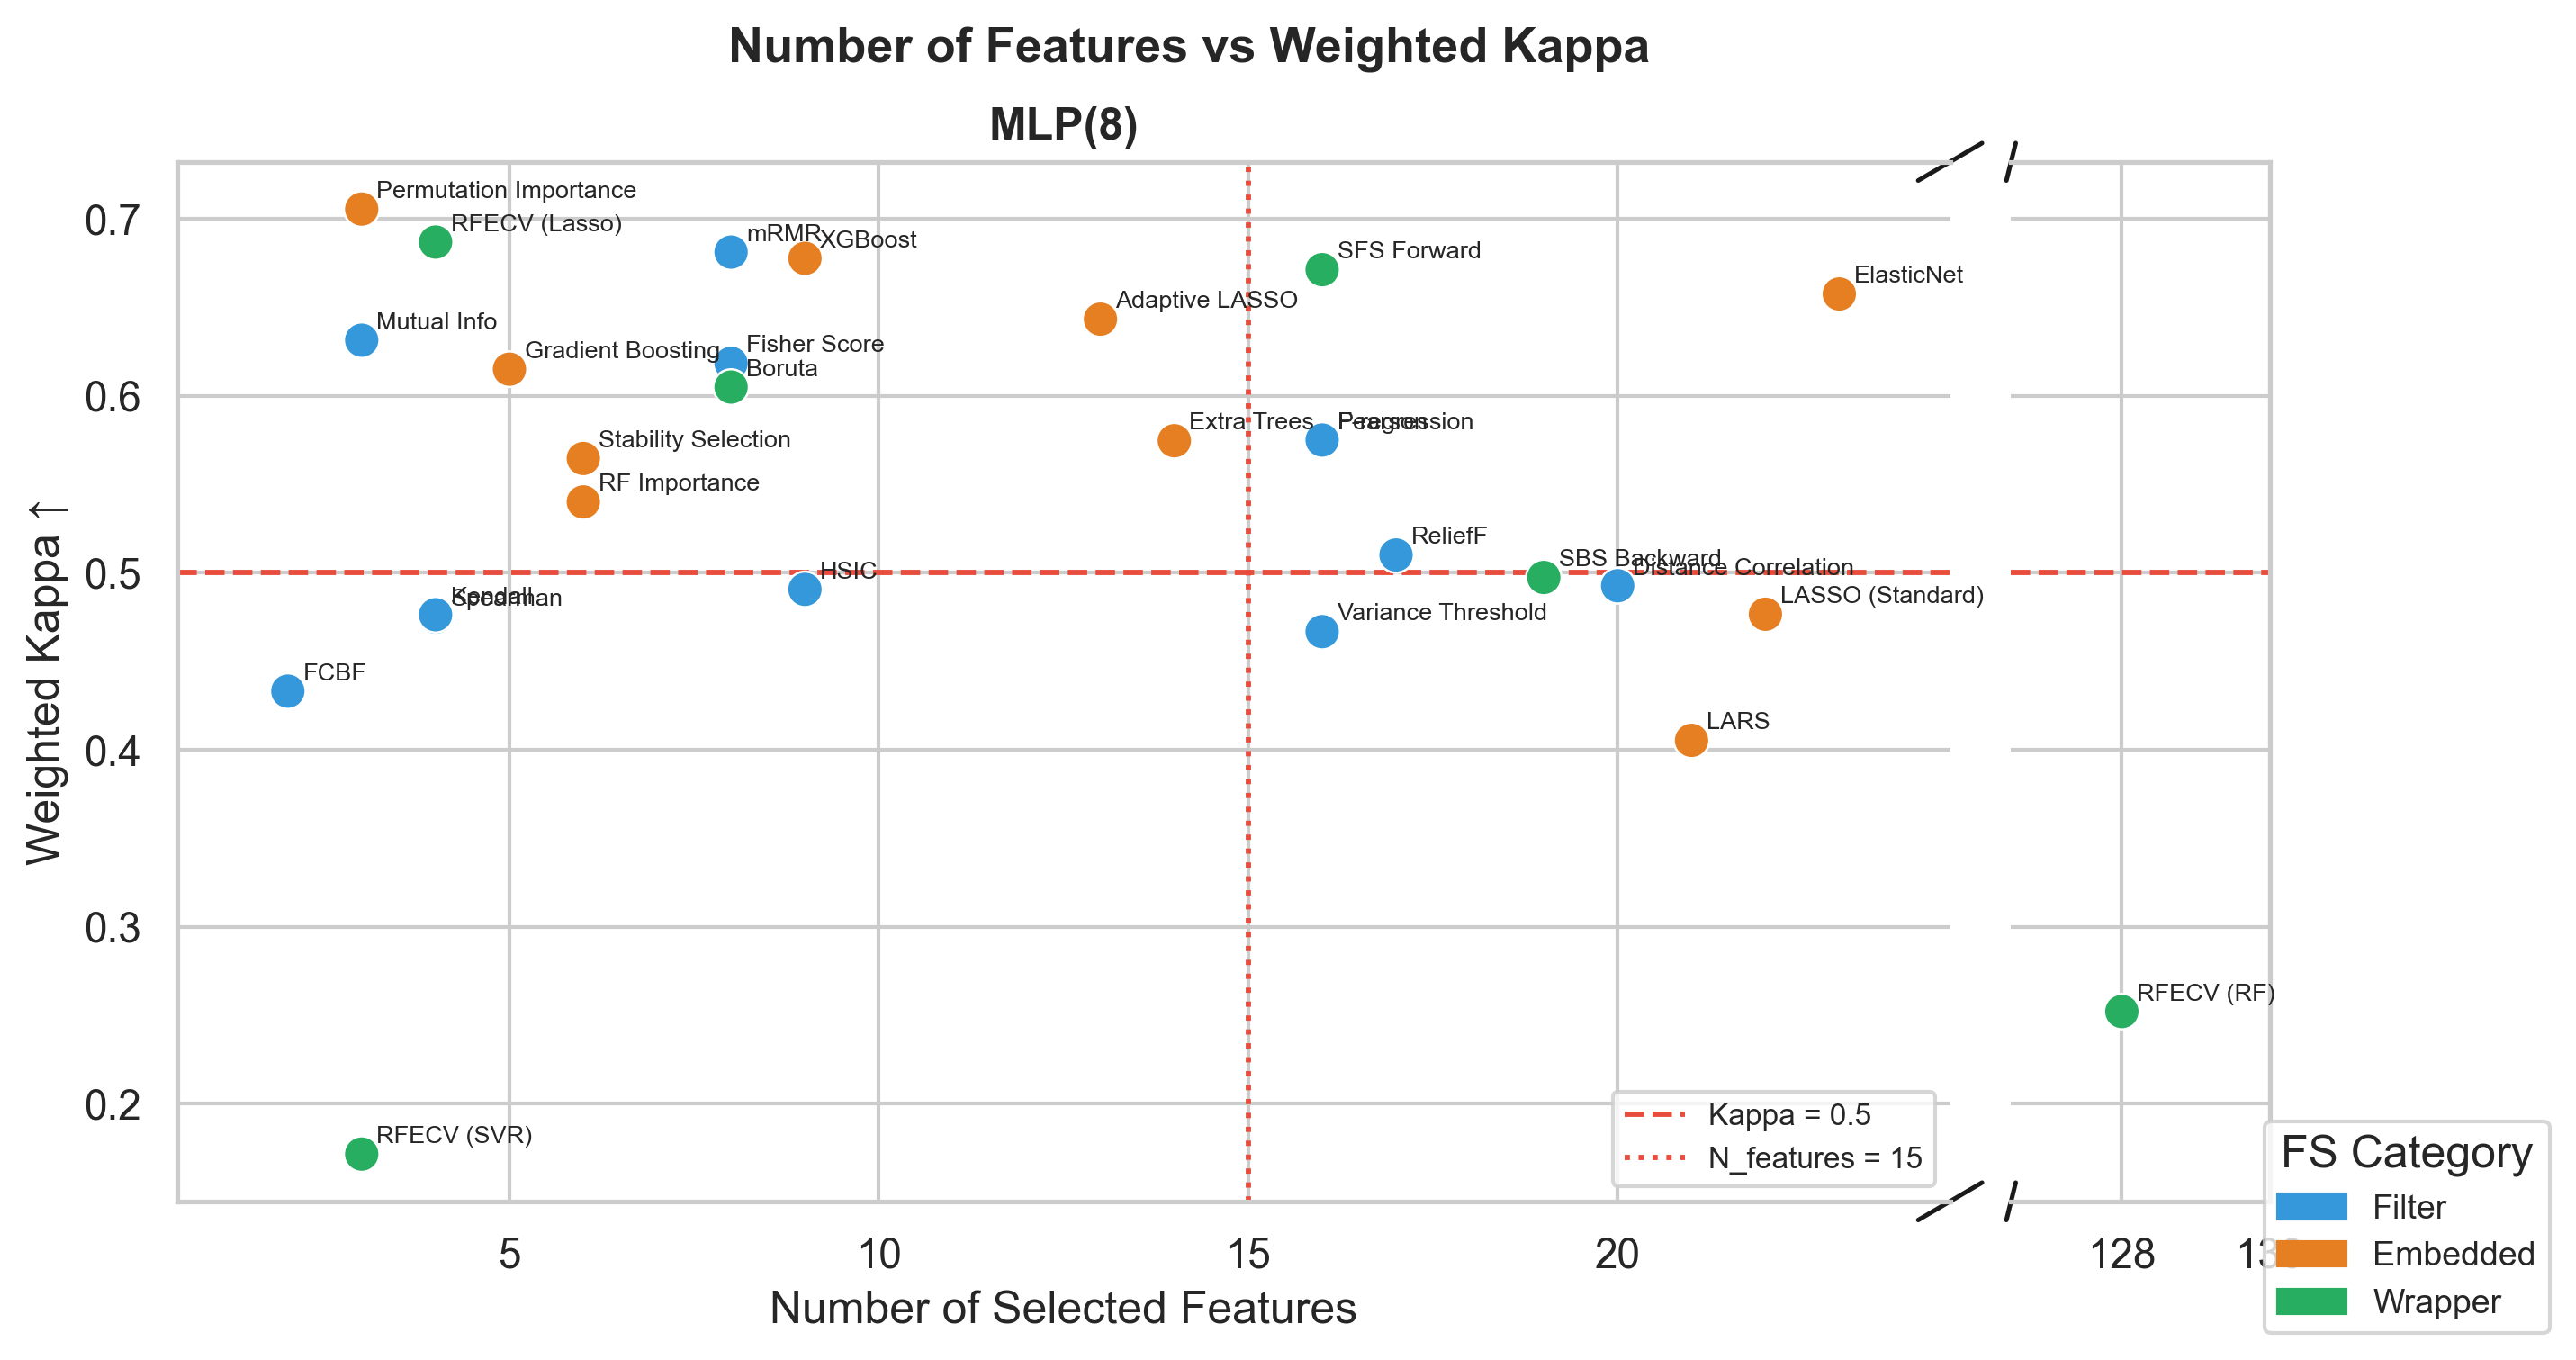
\includegraphics[width=0.85\textwidth,height=0.78\textheight,keepaspectratio]{figD_nfeats_vs_kappa.png}\\
    \scriptsize Red lines = Stage 5 filter (Kappa $\ge 0.5$, $N_\mathrm{feat} < 15$); \textbf{17/28} methods pass.
\end{frame}

\begin{frame}
    \frametitle{FS Pipeline: Feature Inclusion Frequency}
    \centering
    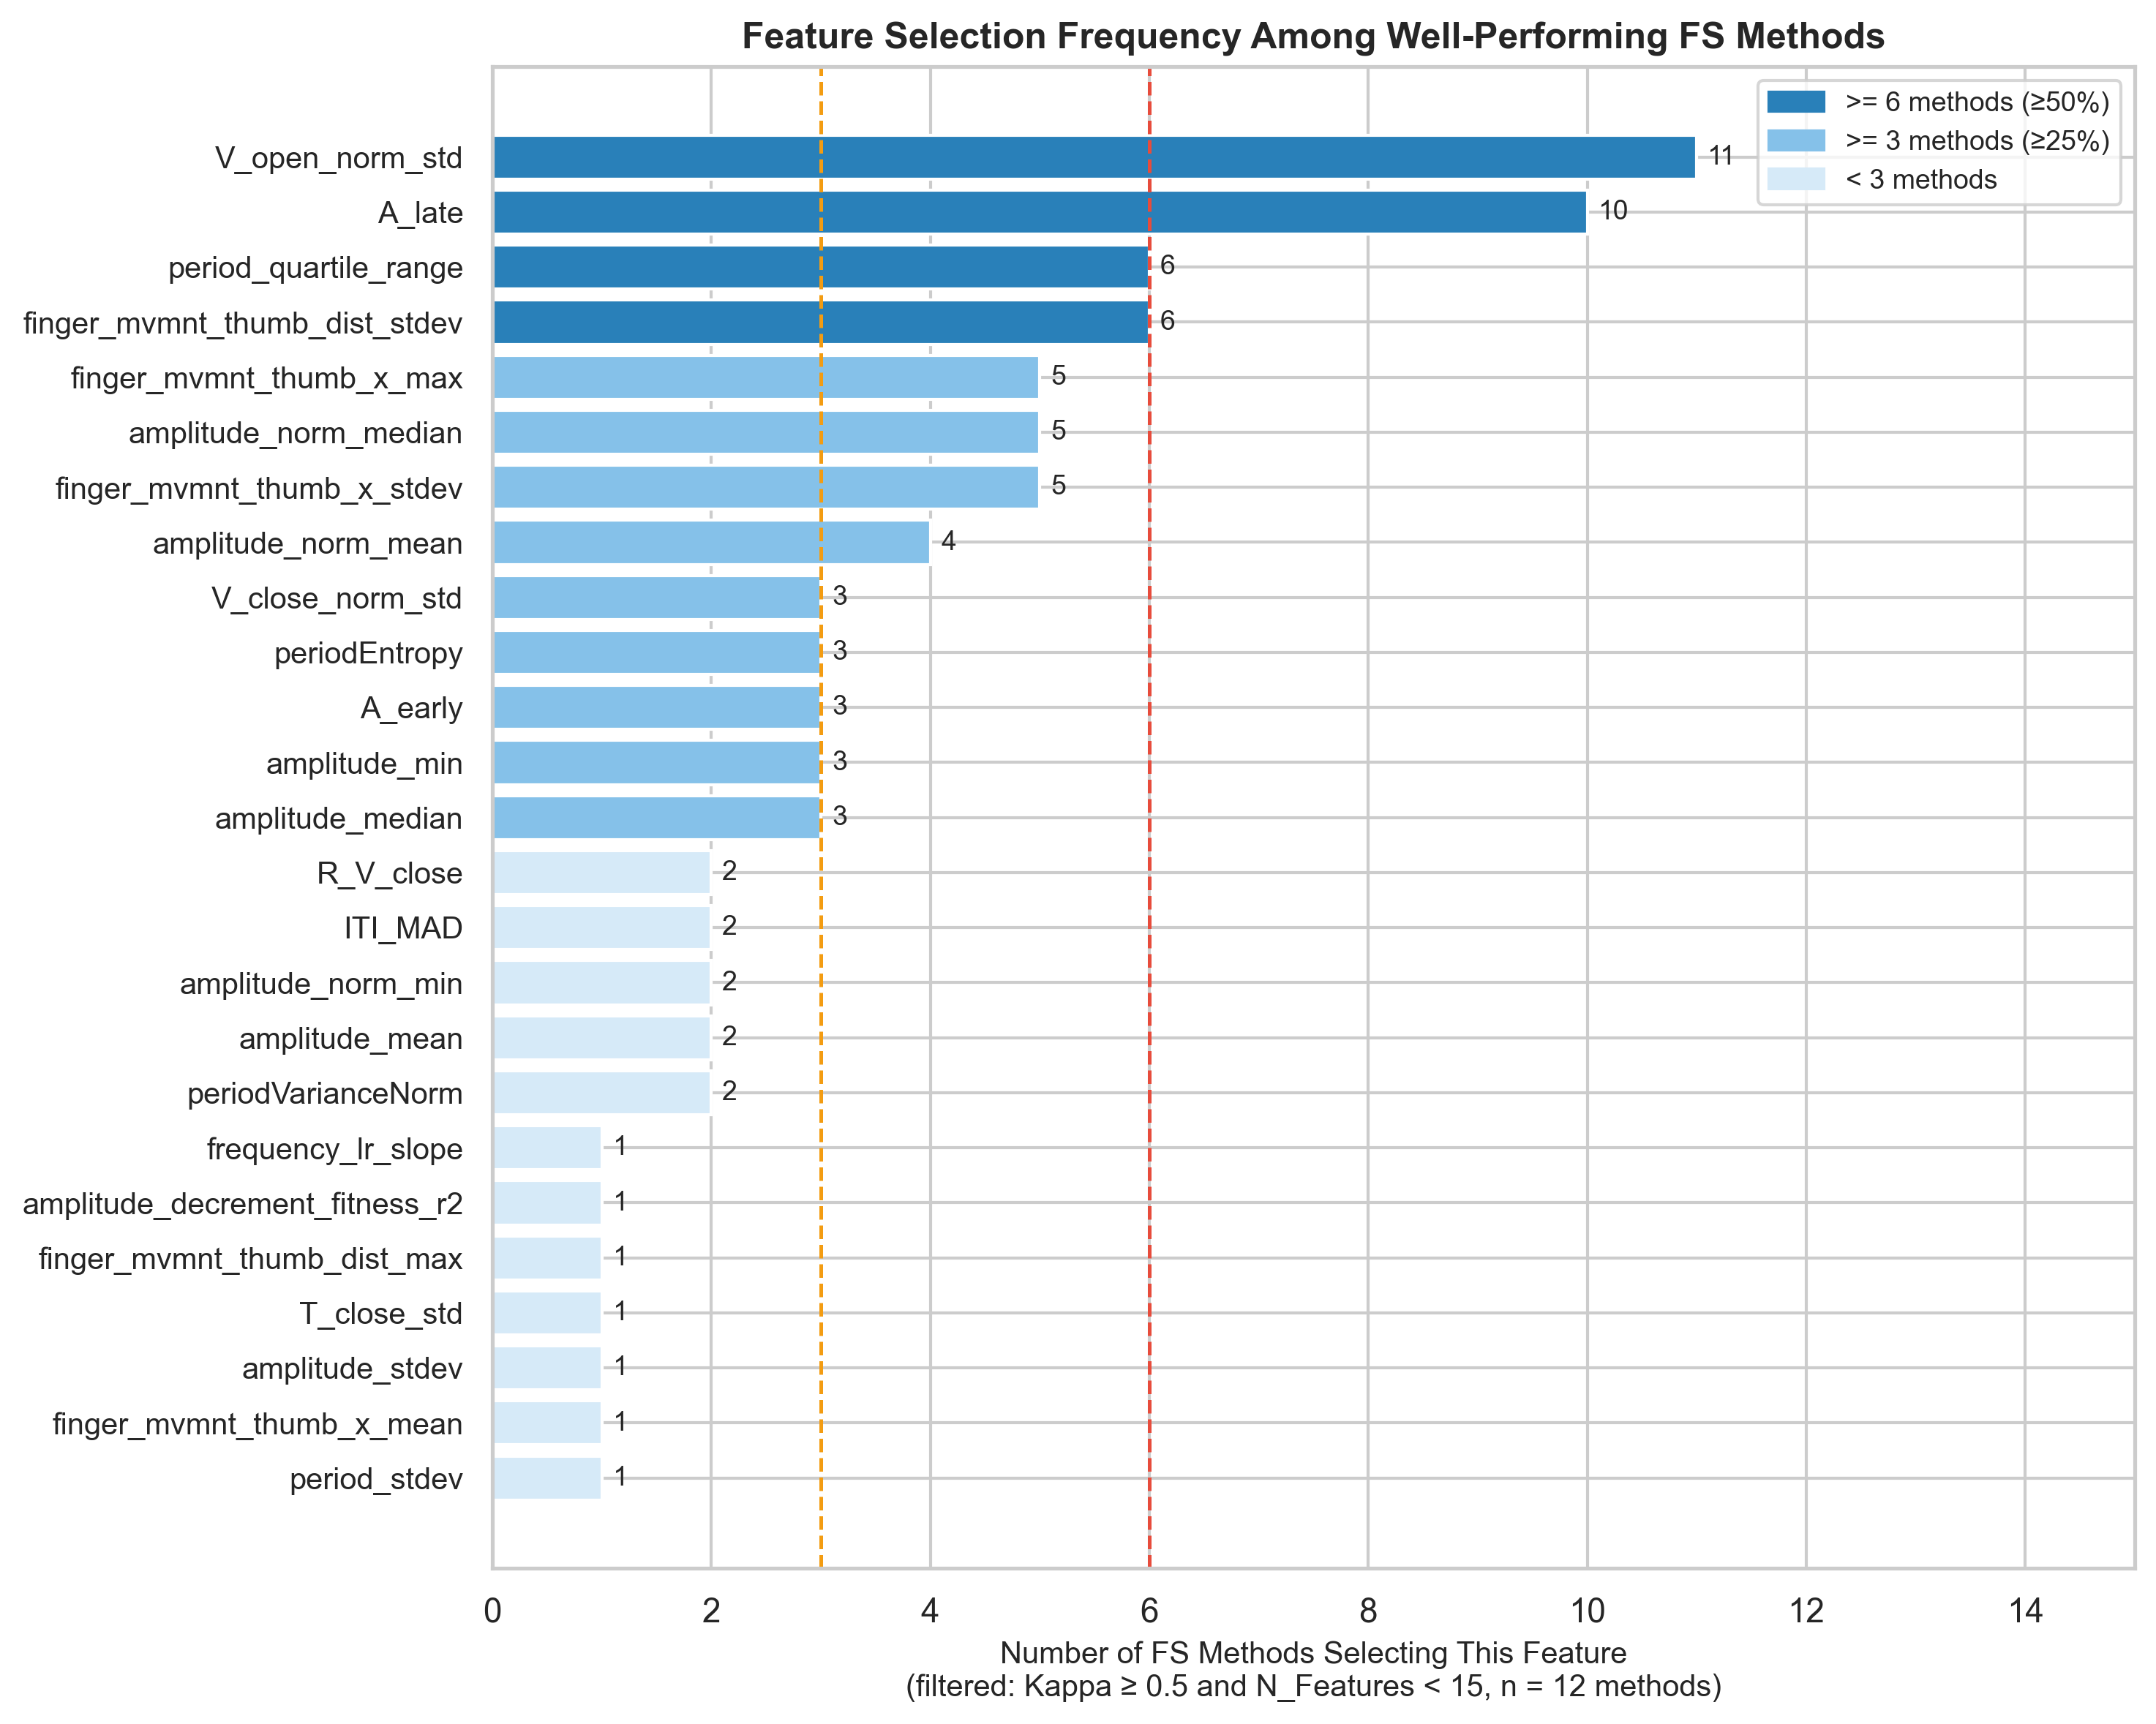
\includegraphics[width=0.62\textwidth,height=0.82\textheight,keepaspectratio]{figE_feature_frequency.png}\\
    \scriptsize Only FS methods passing Stage 5 (17/28) contribute. Features selected by $\ge50\%$ form the final shortlist.
\end{frame}

%%%%%%%%%%%%%%%%%%%%%%%%%%%%%%%%%%%%%%%%%%%%%%%%%%%%%
\begin{frame}
    \frametitle{Wrapper vs.\ MLP Prediction: Internal Score vs.\ Feature Quality}
    \scriptsize
    Wrapper methods produce internal CV predictions $\hat{\mathbf{y}}_\text{wrap}$
    \emph{using their own estimator}; the standardised MLP on the same $\mathcal{S}$ gives
    $\hat{\mathbf{y}}_\text{MLP}$.\\[0.4em]
    \begin{columns}[T]
        \column{0.50\textwidth}
        \textbf{Compare residuals} (sorted by $y_i$):
        \[
            \hat{y}_{\text{wrap},i} - \bar{y}
            \quad \text{vs} \quad
            \hat{y}_{\text{MLP},i} - \bar{y}
        \]
        \vspace{0.3em}
        \textbf{What a large gap means:}
        \begin{itemize}\setlength\itemsep{0.2em}
            \item Wrap bad, MLP \textbf{good}: features are genuinely informative
                  but wrapper's estimator misjudges them\\
                  $\to$ selection driven by noise risk
            \item Wrap good, MLP \textbf{bad}: wrapper overfits to its own estimator
            \item Small gap: internal score faithfully reflects subset quality
        \end{itemize}
        \vspace{0.3em}
        Motivates using a \textbf{fixed MLP} as the uniform yardstick.

        \column{0.48\textwidth}
        \centering
        \vspace{0.5em}
        {\color{gray}\rule{0.9\textwidth}{0.4pt}}\\[0.3em]
        \textit{\footnotesize Figure: per-session residuals\\[0.2em]
        $\hat{y}_{\text{wrap}} - \bar{y}$ \textcolor{blue}{(blue)}\\
        vs $\hat{y}_{\text{MLP}} - \bar{y}$ \textcolor{orange!80!black}{(orange)}\\
        for each of the 5 wrapper methods.\\[0.5em]
        \textnormal{(to be generated from FS pipeline logs)}}\\[0.3em]
        {\color{gray}\rule{0.9\textwidth}{0.4pt}}
    \end{columns}
\end{frame}

\begin{frame}
    \frametitle{Experimental Setup}
    \begin{itemize}
        \item \textbf{Dataset}: 53 finger tapping sessions from 16 PD subjects.
        \item \textbf{Ground Truth}: Consensus score = average of two neurologists' ratings.
        \item \textbf{Input}: First 10 taps trajectory data extracted via CoTracker.
        \item \textbf{Prompt Strategies}:
        \begin{itemize}
            \item \textbf{ZS}: MDS-UPDRS criteria + trajectory data only.
            \item \textbf{FS}: Additional example feature sets from concordant sessions.
        \end{itemize}
        \item \textbf{Evaluation Protocol}:
        \begin{itemize}
            \item 10 independent evaluations per session per model.
            \item Final score = median of 10 evaluations.
        \end{itemize}
    \end{itemize}
\end{frame}


\begin{frame}
    \frametitle{Evaluation Metrics}
    \begin{itemize}
        \item \textbf{MAE} (Mean Absolute Error): Average magnitude of scoring errors. $\downarrow$
        \item \textbf{RMSE} (Root Mean Squared Error): Penalizes large deviations. $\downarrow$
        \item \textbf{Pearson Correlation}: Linear association with ground truth. $\uparrow$
        \item \textbf{Weighted Kappa}: Ordinal agreement penalizing distant disagreements. $\uparrow$
        \item \textbf{Wasserstein Distance}: Distribution-level scoring agreement. $\downarrow$
        \item \textbf{Stability}: Average SD across 10 evaluations per session. $\downarrow$
        \item \textbf{Accuracy (ACC)}: Fraction of exactly correct predictions (after rounding). $\uparrow$
        \item \textbf{Macro Recall}: Per-class recall averaged across all score classes (0--4). $\uparrow$
    \end{itemize}
    \vspace{0.3em}
    Additionally, \textbf{binary classification} (Normal=0 vs.\ Abnormal$\geq$1): ACC, Recall, Precision, F1.\\
    All metrics reported with \textbf{95\% bootstrap CI} (2,000 replicates).
\end{frame}


%%%%%%%%%%%%%%%%%%%%%%%%%%%%%%%%%%%%%%%%%%%%%%%%%%%%%
\section{Results}



\begin{frame}
    \frametitle{Performance Summary Table}
    {\color{black}
    {\tiny
    \begin{table}
        \centering
        \setlength{\tabcolsep}{3.5pt}
        \begin{tabular}{lcccccccc}
        \toprule
        \textbf{Model} & \textbf{ACC $\uparrow$} & \textbf{AAcc $\uparrow$} & \textbf{MAE $\downarrow$} & \textbf{RMSE $\downarrow$} & \textbf{Corr $\uparrow$} & \textbf{Kappa $\uparrow$} & \textbf{WD $\downarrow$} & \textbf{Stab $\downarrow$} \\
        \midrule
        deepseek-r1\_32b FS & \cellcolor{green!15}\textbf{56.6\%} & 90.6\% & \cellcolor{green!15}\textbf{0.53} & 0.85 & \cellcolor{green!15}\textbf{0.56} & \cellcolor{green!15}\textbf{0.54} & 0.26 & 0.449 \\
        deepseek-r1\_32b ZS & 37.7\% & \cellcolor{red!15}81.1\% & \cellcolor{red!15}0.81 & \cellcolor{red!15}1.09 & 0.37 & 0.30 & \cellcolor{red!15}0.58 & 0.658 \\
        deepseek-r1\_70b FS & 43.4\% & 90.6\% & 0.66 & 0.92 & 0.48 & 0.48 & 0.25 & 0.421 \\
        deepseek-r1\_70b ZS & 41.5\% & 98.1\% & 0.60 & 0.80 & 0.48 & 0.43 & 0.38 & 0.421 \\
        qwen3\_30b FS       & 49.1\% & 88.7\% & 0.62 & 0.92 & 0.46 & 0.45 & 0.17 & 0.786 \\
        qwen3\_30b ZS       & 45.3\% & \cellcolor{red!15}81.1\% & 0.74 & 1.06 & \cellcolor{red!15}0.30 & 0.30 & \cellcolor{green!15}\textbf{0.06} & \cellcolor{red!15}0.876 \\
        qwen2.5\_7b FS      & \cellcolor{red!15}32.1\% & \cellcolor{green!15}\textbf{100.0\%} & 0.68 & 0.82 & 0.52 & 0.45 & 0.45 & 0.620 \\
        qwen2.5\_7b ZS      & 35.8\% & 98.1\% & 0.66 & 0.84 & 0.38 & \cellcolor{red!15}0.28 & 0.55 & 0.774 \\
        qwen2.5\_32b FS     & 49.1\% & 88.7\% & 0.66 & 1.02 & 0.46 & 0.43 & 0.40 & 0.405 \\
        qwen2.5\_32b ZS     & 49.1\% & 98.1\% & \cellcolor{green!15}\textbf{0.53} & \cellcolor{green!15}\textbf{0.75} & 0.55 & 0.50 & 0.34 & 0.588 \\
        qwen2.5\_72b FS     & 50.9\% & 88.7\% & 0.64 & 1.01 & 0.48 & 0.44 & 0.42 & 0.314 \\
        qwen2.5\_72b ZS     & 43.4\% & 98.1\% & 0.58 & 0.79 & 0.50 & 0.45 & 0.32 & 0.423 \\
        Gemini3 Flash FS    & 39.6\% & 86.8\% & 0.77 & \cellcolor{red!15}1.09 & 0.42 & 0.39 & 0.32 & \cellcolor{green!15}\textbf{0.148} \\
        Gemini3 Flash ZS    & 49.1\% & 86.8\% & 0.66 & 1.00 & 0.49 & 0.37 & \cellcolor{red!15}0.58 & 0.331 \\
        \midrule
        \rowcolor{yellow!12}
        Doctor (Tan)        & 60.4\% & 100.0\% & 0.40 & 0.63 & 0.72 & 0.69 & 0.25 & 0.000 \\
        \rowcolor{yellow!12}
        Doctor (Chien)      & 64.2\% & 100.0\% & 0.36 & 0.60 & 0.85 & 0.83 & 0.32 & 0.000 \\
        \rowcolor{gray!12}
        Random (uniform)    & 3.8\% & 32.8\% & 1.46 & 1.82 & $\sim$0.00 & $\sim$0.00 & 0.74 & -- \\
        \rowcolor{gray!12}
        Random (proportional) & 17.2\% & 55.7\% & 0.96 & 1.27 & $\sim$0.00 & $\sim$0.00 & 0.13 & -- \\
        \bottomrule
        \end{tabular}
    \end{table}
    }
    }
    \vspace{0.3em}
    \footnotesize{AAcc = Acceptable Accuracy ($|$error$|\leq 1$).\\
    \colorbox{yellow!12}{Yellow} = Doctor baselines (each doctor vs.\ consensus). \colorbox{gray!12}{Gray} = Random baselines (10k trials).}
\end{frame}


\begin{frame}
    \frametitle{Binary Classification: Normal (0) vs Abnormal ($\geq$1)}
    {\color{black}{\small
    \begin{table}
        \centering
        \begin{tabular}{llcccc}
        \toprule
        \textbf{Type} & \textbf{Model} & \textbf{ACC $\uparrow$} & \textbf{Recall $\uparrow$} & \textbf{Precision $\uparrow$} & \textbf{F1 $\uparrow$} \\
        \midrule
        \rowcolor{gray!10}
        ML & RandomForest        & 79.2\% & 89.2\% & 82.5\% & 85.7\% \\
        \rowcolor{gray!10}
        ML & XGBoost             & 73.6\% & 89.2\% & 76.7\% & 82.5\% \\
        \midrule
        \rowcolor{gray!10}
        Dallen & Gemini3 Flash ZS & 75.5\% & 73.2\% & \cellcolor{green!20}\textbf{93.8\%} & 82.2\% \\
        \midrule
        LLM & DS-R1-32b FS   & \cellcolor{green!20}\textbf{86.8\%} & \cellcolor{green!20}\textbf{100.0\%} & 85.4\% & \cellcolor{green!20}\textbf{92.1\%} \\
        LLM & DS-R1-32b ZS   & 77.4\% & \cellcolor{green!20}\textbf{100.0\%} & 77.4\% & 87.2\% \\
        \midrule
        \rowcolor{yellow!12}
        Doctor & Tan vs Consensus & 84.9\% & 100.0\% & \cellcolor{green!20}\textbf{93.2\%} & 91.1\% \\
        \rowcolor{yellow!12}
        Doctor & Chien vs Consensus & 90.6\% & 90.2\% & 92.5\% & 93.7\% \\
        \rowcolor{gray!12}
        Random & Uniform        & 66.4\% & 80.0\% & 78.6\% & 78.6\% \\
        \rowcolor{gray!12}
        Random & Proportional   & 64.9\% & 77.4\% & 77.2\% & 77.2\% \\
        \bottomrule
        \end{tabular}
    \end{table}
    }}
    \vspace{0.2em}
    \footnotesize{
    TML: Leave-One-Out CV (LOO-CV).\\
    LLMs surpass both TML and random baselines; DS-R1-32b FS approaches doctor-level binary detection.}
\end{frame}


\begin{frame}
    \frametitle{Baseline Context: Why Doctor \& Random Baselines Matter}
    \begin{itemize}
        \item \textbf{Upper bound --- Doctor baseline}:
        \begin{itemize}
            \item Each doctor's score vs.\ consensus (average of both doctors).
            \item Doctor (Chien): Kappa = 0.83, Corr = 0.85 --- the \emph{ceiling} for any automated system.
            \item Doctor (Tan): Kappa = 0.69, Corr = 0.72 --- shows inter-rater variability.
        \end{itemize}
        \item \textbf{Lower bound --- Random baseline}:
        \begin{itemize}
            \item Uniform random: Kappa $\approx$ 0.00, MAE = 1.46 --- any model \emph{must} beat this.
            \item Proportional random: MAE = 0.96 --- even matching label distribution yields low accuracy.
        \end{itemize}
        \item \textbf{LLM positioning}:
        \begin{itemize}
            \item Best LLM (DS-R1-32b FS): Kappa = 0.54, sits at \textbf{65\%} of the gap between random and doctor.
            \item All 14 LLM configs clearly surpass random baselines across all metrics.
            \item Gap to doctor level $\approx$ 0.15--0.30 Kappa --- room for improvement.
        \end{itemize}
    \end{itemize}
\end{frame}


\begin{frame}
    \frametitle{Recall Analysis: Binary Classification}
    \begin{itemize}
        \item \textbf{Binary Recall} (Abnormal$\geq$1) is clinically critical:
        \begin{itemize}
            \item Missing an abnormal case (false negative) has greater clinical cost than a false positive.
            \item High binary recall = fewer missed abnormal sessions.
        \end{itemize}
        \item \textbf{Key findings}:
        \begin{itemize}
            \item DS-R1-32b (FS \& ZS) achieves \textbf{100\% recall} --- no abnormal case missed.
            \item Dallen's approach has lower recall (73.2\%) --- misses 11 out of 41 abnormal sessions.
            \item DS-R1-32b FS achieves best balance: highest ACC (86.8\%) with perfect recall.
        \end{itemize}
    \end{itemize}
\end{frame}








%%%%%%%%%%%%%%%%%%%%%%%%%%%%%%%%%%%%%%%%%%%%%%%%%%%%%
\section{Model Agreement Analysis}

\begin{frame}
    \frametitle{Error Distribution per Model}
    \begin{figure}
        \centering
        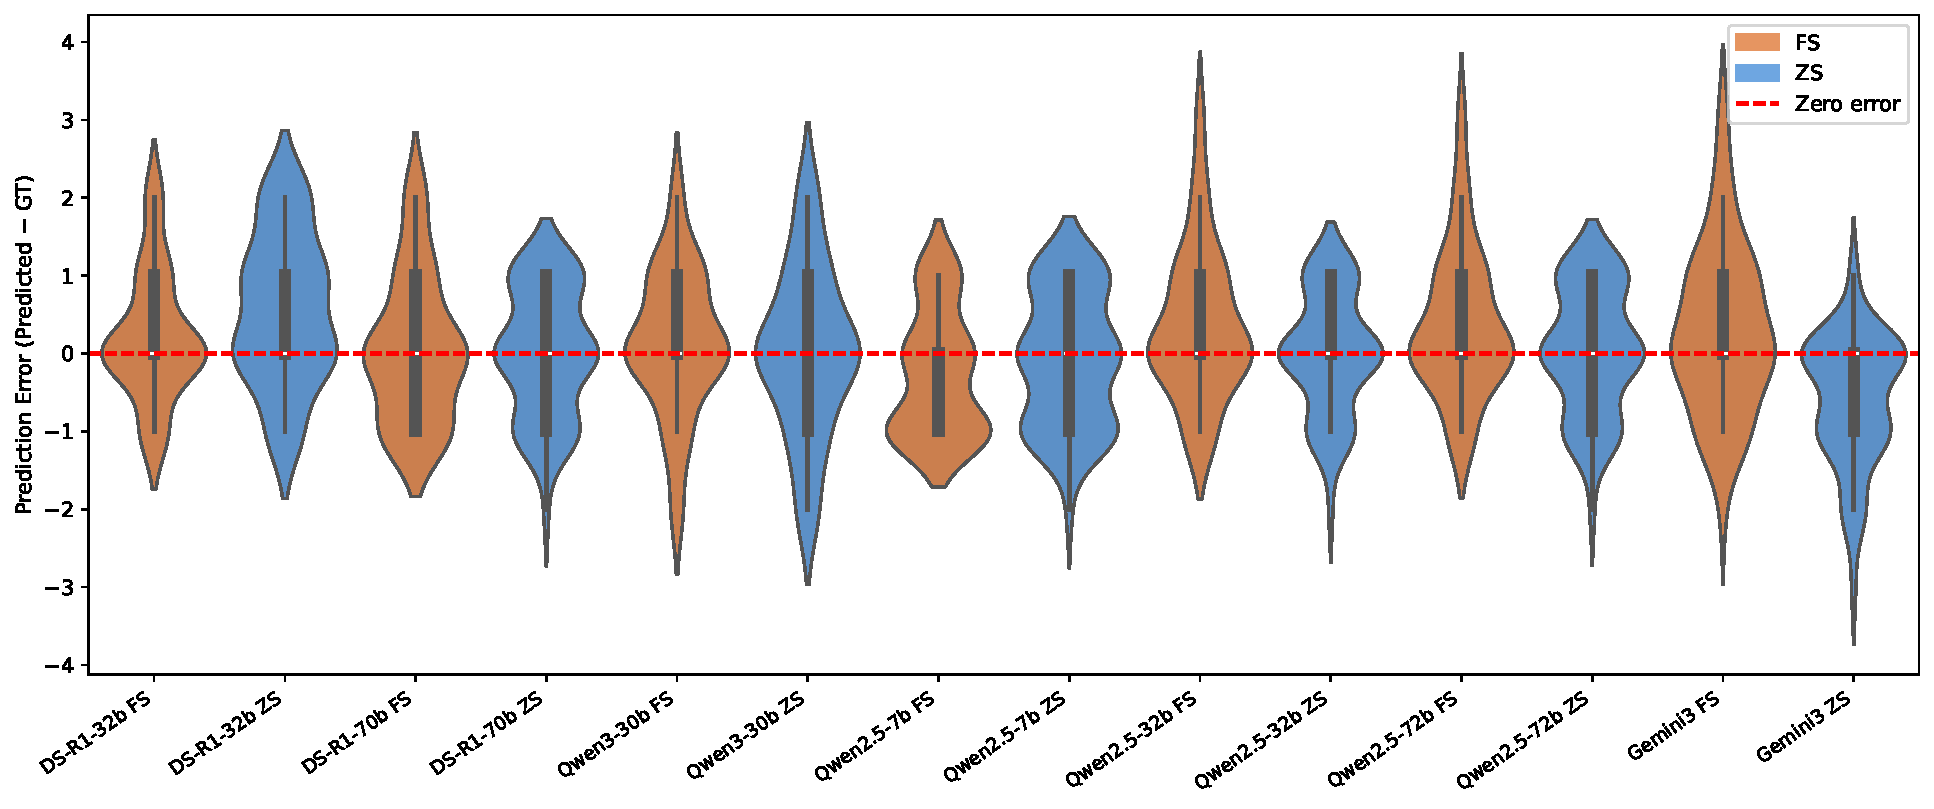
\includegraphics[width=\textwidth, height=0.82\textheight, keepaspectratio]{error_violin.pdf}
    \end{figure}
    \vspace{-0.3em}
    \tiny{Violin width = frequency of that error value. Red dashed line = zero error. Inner box = IQR \& median.}
\end{frame}


\begin{frame}
    \frametitle{Pairwise KS Test: Gemini3 Flash ZS vs All Models}
    {\color{black}{\scriptsize
    \setlength{\tabcolsep}{4pt}
    \begin{table}
        \centering
        \begin{tabular}{lc}
        \toprule
        \textbf{Model} & \textbf{$p$-value} \\
        \midrule
        DS-R1-32b FS    & \cellcolor{red!15}$4.2 \times 10^{-4}$ \\
        DS-R1-32b ZS    & \cellcolor{red!15}$3.8 \times 10^{-6}$ \\
        DS-R1-70b FS    & \cellcolor{red!15}0.008 \\
        DS-R1-70b ZS    & \cellcolor{red!15}0.028 \\
        Gemini3 Flash FS & \cellcolor{red!15}0.002 \\
        qwen2.5\_7b FS  & 0.304 \\
        qwen2.5\_7b ZS  & \cellcolor{red!15}0.049 \\
        qwen2.5\_32b FS & \cellcolor{red!15}$2.8 \times 10^{-5}$ \\
        qwen2.5\_32b ZS & \cellcolor{red!15}0.028 \\
        qwen2.5\_72b FS & \cellcolor{red!15}$7.3 \times 10^{-5}$ \\
        qwen2.5\_72b ZS & \cellcolor{red!15}0.028 \\
        qwen3\_30b FS   & \cellcolor{red!15}0.004 \\
        qwen3\_30b ZS   & \cellcolor{red!15}0.002 \\
        \bottomrule
        \end{tabular}
    \end{table}
    }}
    \vspace{0.3em}
    \footnotesize{Two-sample KS test on prediction error distributions.\\
    \colorbox{red!15}{Red}: $p < 0.05$ --- Gemini3 Flash ZS is significantly different from 12 out of 13 models, indicating it is a distributional outlier.}
\end{frame}


%%%%%%%%%%%%%%%%%%%%%%%%%%%%%%%%%%%%%%%%%%%%%%%%%%%%%
\section{Discussion}


\begin{frame}
    \frametitle{Model Size Effect: Qwen2.5 Scaling (ZS)}
    {\color{black}{\small
    \begin{table}
        \centering
        \setlength{\tabcolsep}{5pt}
        \begin{tabular}{lccccc}
        \toprule
        \textbf{Model} & \textbf{ACC} & \textbf{AAcc} & \textbf{MAE} & \textbf{Kappa} & \textbf{Corr} \\
        \midrule
        qwen2.5\_7b ZS  & 35.8\% & 98.1\% & 0.66 & 0.28 & 0.38 \\
        qwen2.5\_32b ZS & \cellcolor{green!15}\textbf{49.1\%} & 98.1\% & \cellcolor{green!15}\textbf{0.53} & \cellcolor{green!15}\textbf{0.50} & \cellcolor{green!15}\textbf{0.55} \\
        qwen2.5\_72b ZS & 43.4\% & 98.1\% & 0.58 & 0.45 & 0.50 \\
        \bottomrule
        \end{tabular}
    \end{table}
    }}
    \vspace{0.5em}
    \begin{itemize}
        \item 7b $\rightarrow$ 32b: clear improvement across all metrics.
        \item 32b $\rightarrow$ 72b: \textbf{performance drops} --- larger is not always better.
        \item 32b appears to be the optimal size for this task under ZS.
        \item AAcc stays at 98.1\% across all sizes --- scaling affects \emph{exact} accuracy, not tolerance.
    \end{itemize}
\end{frame}


\begin{frame}
    \frametitle{FS vs ZS: Effect Across All Models}
    \begin{columns}
        \begin{column}{0.48\textwidth}
            {\color{black}{\scriptsize
            \setlength{\tabcolsep}{3pt}
            \begin{tabular}{lcccc}
            \toprule
            \textbf{Model} & \textbf{$\Delta$Kappa} & \textbf{$\Delta$MAE} & \textbf{$\Delta$AAcc} & \textbf{Dir.} \\
            \midrule
            deepseek-r1\_32b & $+$0.24 & $-$0.28 & $-$7.5\% & \cellcolor{green!15}FS \\
            qwen3\_30b       & $+$0.15 & $-$0.12 & $+$7.6\% & \cellcolor{green!15}FS \\
            qwen2.5\_7b      & $+$0.17 & $-$0.02 & $+$1.9\% & \cellcolor{green!15}FS \\
            deepseek-r1\_70b & $+$0.05 & $-$0.06 & $-$7.5\% & \cellcolor{green!15}FS \\
            Gemini3 Flash    & $+$0.02 & $-$0.11 & $\ $0\% & mixed \\
            qwen2.5\_72b     & $-$0.01 & $+$0.06 & $-$9.4\% & \cellcolor{red!15}ZS \\
            qwen2.5\_32b     & $-$0.07 & $+$0.13 & $-$9.4\% & \cellcolor{red!15}ZS \\
            \bottomrule
            \end{tabular}
            }}
            \vspace{0.5em}\\
            \tiny{$\Delta$ = FS $-$ ZS. \colorbox{green!15}{Green} = FS better; \colorbox{red!15}{Red} = ZS better.}
        \end{column}
        \begin{column}{0.52\textwidth}
            \begin{figure}
                \centering
                
\includegraphics[width=\textwidth]{1b_fewshot_zeroshot_delta.pdf}
                \caption*{\tiny Green = few-shot better; Red = zero-shot better}
            \end{figure}
        \end{column}
    \end{columns}
\end{frame}


\begin{frame}
    \frametitle{Reasoning Distillation: Numerical Comparison}
    {\color{black}{\tiny
    \begin{table}
        \centering
        \begin{tabular}{llccccc}
        \toprule
        \textbf{Model} & \textbf{Prompt} & \textbf{MAE $\downarrow$} & \textbf{Kappa $\uparrow$} & \textbf{Corr $\uparrow$} & \textbf{WD $\downarrow$} & \textbf{Stab $\downarrow$} \\
        \midrule
        Qwen2.5-32b (base) & FS  & 0.66 {\tiny[0.47, 0.87]} & 0.43 {\tiny[0.15, 0.64]} & 0.46 {\tiny[0.18, 0.67]} & 0.40 {\tiny[0.21, 0.64]} & 0.405 \\
        Qwen2.5-32b (base) & ZS & \cellcolor{green!20}\textbf{0.53} {\tiny[0.38, 0.66]} & 0.50 {\tiny[0.33, 0.64]} & 0.55 {\tiny[0.37, 0.69]} & \cellcolor{green!20}\textbf{0.34} {\tiny[0.17, 0.51]} & 0.588 \\
        DS-R1-32b (distilled) & FS  & \cellcolor{green!20}\textbf{0.53} {\tiny[0.36, 0.72]} & \cellcolor{green!20}\textbf{0.54} {\tiny[0.29, 0.71]} & \cellcolor{green!20}\textbf{0.56} {\tiny[0.32, 0.73]} & 0.26 {\tiny[0.17, 0.47]} & 0.449 \\
        DS-R1-32b (distilled) & ZS & 0.81 {\tiny[0.60, 1.02]} & 0.30 {\tiny[0.10, 0.47]} & 0.37 {\tiny[0.13, 0.56]} & 0.58 {\tiny[0.36, 0.83]} & 0.658 \\
        \bottomrule
        \end{tabular}
    \end{table}
    }}
    \vspace{0.2em}
    \footnotesize{
    $\Delta$Kappa(distilled FS vs base FS): $+0.11$ \quad $\Delta$Kappa(distilled ZS vs base ZS): $-0.20$}
    \vspace{0.3em}
    \begin{itemize}\setlength{\itemsep}{2pt}
        \footnotesize
        \item Distilled + FS: best Kappa (0.54) and Corr (0.56) --- few-shot examples anchor CoT reasoning.
        \item Distilled + ZS: worst MAE (0.81) and Kappa (0.30) --- unconstrained CoT drifts without examples.
    \end{itemize}
\end{frame}



\begin{frame}
    \frametitle{Effect of Reasoning Distillation}
    \begin{columns}[c]
        \begin{column}{0.44\textwidth}
            \small
            \begin{itemize}\setlength{\itemsep}{4pt} 
                \item DeepSeek-R1-32b $=$ \textbf{Qwen2.5-32b} fine-tuned on DeepSeek-R1 CoT traces (RL reasoning distillation).
                \item \textbf{FS}: large gains (Kappa $+$0.11, MAE $-$0.13) --- CoT anchored by examples.
                \item \textbf{ZS}: distillation \emph{hurts} (Kappa $-$0.20, MAE $+$0.28) --- unconstrained CoT drifts.
                \item \textbf{Implication}: Reasoning-distilled models need FS to realise potential.
            \end{itemize}
        \end{column}
        \begin{column}{0.56\textwidth}
            \begin{figure}
                \centering
                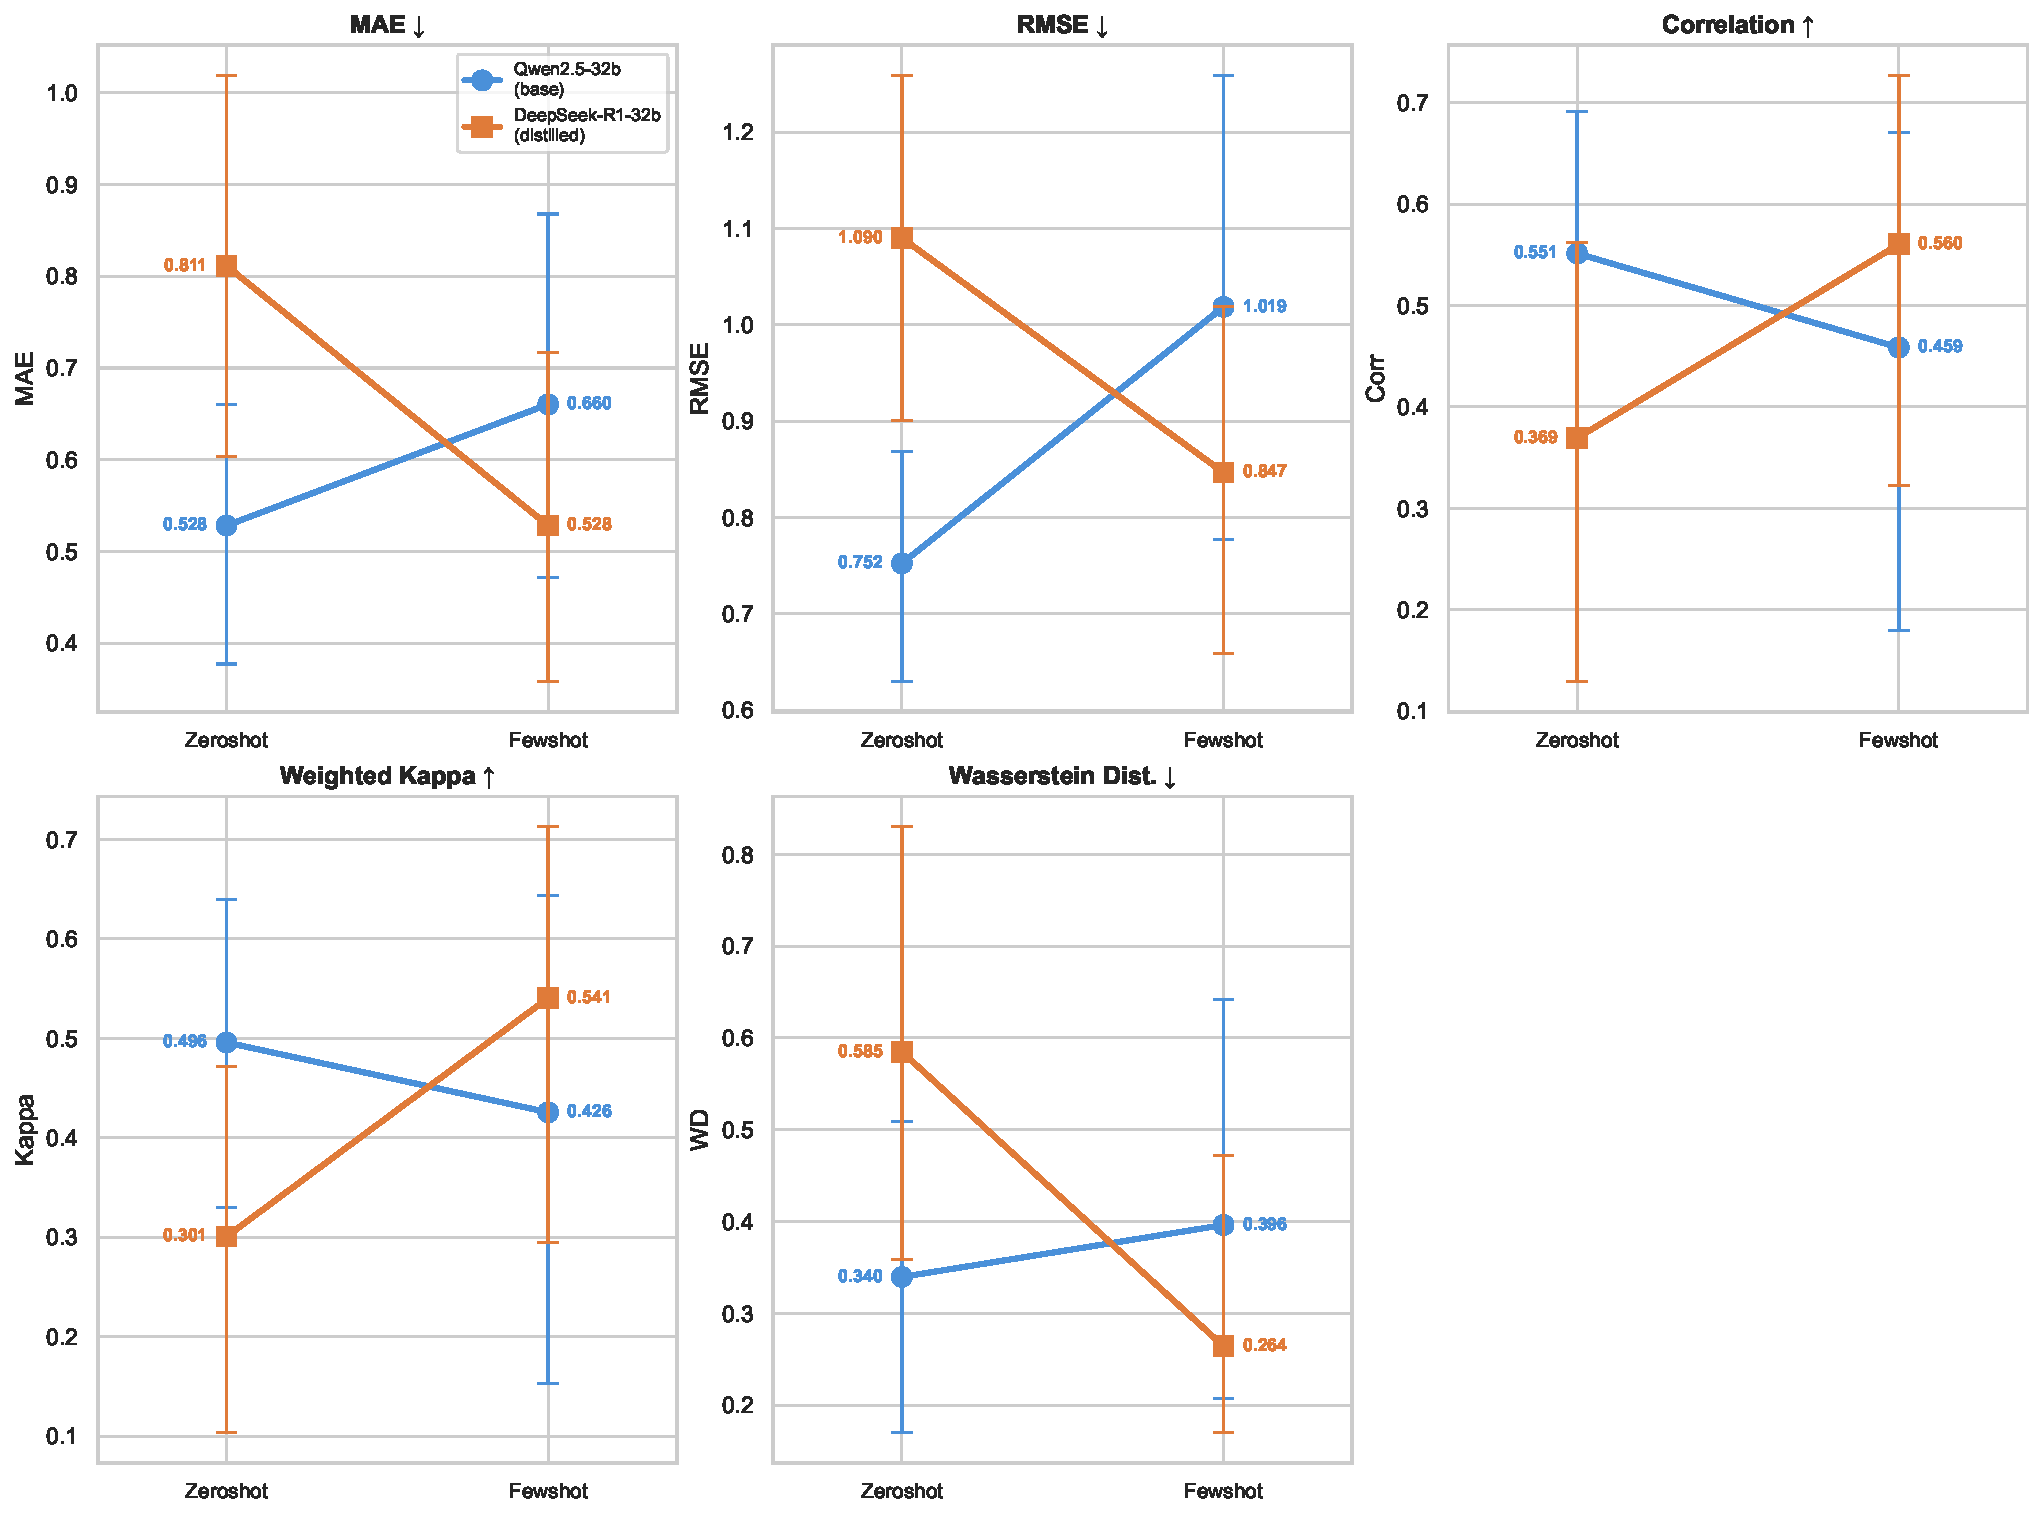
\includegraphics[width=\textwidth]{3a_distill_interaction.pdf}
                \caption*{\tiny Lines cross between Zeroshot and Fewshot, revealing the interaction effect.}
            \end{figure}
        \end{column}
    \end{columns}
\end{frame}


%%%%%%%%%%%%%%%%%%%%%%%%%%%%%%%%%%%%%%%%%%%%%%%%%%%%%

\begin{frame}
    \frametitle{Feature-Based vs Trajectory-Only Comparison}
    \footnotesize{This work: feature extraction + reduced tokens. Dallen: raw trajectory (full tokens, ZS). Same 53 sessions.}
    \vspace{0.3em}
    {\footnotesize
    \setlength{\tabcolsep}{3.5pt}
    \begin{table}
        \centering
        \begin{tabular}{llccccccc}
        \toprule
        & \textbf{Model} & \textbf{ACC $\uparrow$} & \textbf{AAcc $\uparrow$} & \textbf{MAE $\downarrow$} & \textbf{Corr $\uparrow$} & \textbf{Kappa $\uparrow$} & \textbf{WD $\downarrow$} & \textbf{Stab $\downarrow$} \\
        \midrule
        Dallen & Gemini3 Flash (ZS) & 45.3\% & 88.7\% & 0.70 & 0.44 & 0.39 & 0.49 & 0.41 \\
        \midrule
        This work & Gemini3 Flash ZS & 49.1\% & 86.8\% & 0.66 & 0.49 & 0.37 & 0.58 & \cellcolor{green!15}\textbf{0.331} \\
        This work & DS-R1-32b FS & \cellcolor{green!15}\textbf{56.6\%} & 90.6\% & \cellcolor{green!15}\textbf{0.53} & \cellcolor{green!15}\textbf{0.56} & \cellcolor{green!15}\textbf{0.54} & \cellcolor{green!15}\textbf{0.26} & 0.449 \\
        This work & Qwen2.5-32b ZS & 49.1\% & \cellcolor{green!15}\textbf{98.1\%} & \cellcolor{green!15}\textbf{0.53} & 0.55 & 0.50 & 0.34 & 0.588 \\
        \midrule
        \rowcolor{yellow!12}
        Baseline & Doctor (Chien) & 64.2\% & 100.0\% & 0.36 & 0.85 & 0.83 & 0.32 & 0.000 \\
        \rowcolor{gray!12}
        Baseline & Random (uniform) & 3.8\% & 32.8\% & 1.46 & $\sim$0 & $\sim$0 & 0.74 & -- \\
        \bottomrule
        \end{tabular}
    \end{table}
    }
    \vspace{0.3em}
    \begin{itemize}\setlength{\itemsep}{2pt}
        \footnotesize
        \item \textbf{Same model (Gemini3 Flash)}: feature extraction improves ACC 45.3\%$\to$49.1\%, Corr 0.44$\to$0.49.
        \item DS-R1-32b FS achieves best overall: ACC 56.6\%, Kappa 0.54 --- far exceeding trajectory-only.
        \item Feature extraction reduces input tokens $\sim$28$\times$ --- lower cost, faster inference, compatible with smaller context-window models.
    \end{itemize}
\end{frame}


%%%%%%%%%%%%%%%%%%%%%%%%%%%%%%%%%%%%%%%%%%%%%%%%%%%%%
\section{Conclusion}

\begin{frame}
    \frametitle{Conclusion}
    \begin{itemize}
        \item All models achieve MAE 0.53--0.81; \textbf{multiple LLM families} are capable of MDS-UPDRS FT scoring from trajectory data.
        \item \textbf{Best configurations}: DeepSeek-R1-32b FS (Kappa 0.54, Corr 0.56), Qwen2.5-32b ZS (MAE 0.53, RMSE 0.75).
        \item \textbf{Reasoning distillation is prompt-sensitive}: DeepSeek-R1-32b (= Qwen2.5-32b + CoT distillation) gains $+$0.11 Kappa with FS but loses $-$0.20 Kappa without examples --- unconstrained chain-of-thought drifts.
        \item \textbf{Scaling benefit depends on base architecture and prompt strategy}: not a universal rule.
        \item \textbf{Stability varies widely}: 0.148 (Gemini) to 0.876 (Qwen3-30b ZS); consistency must be evaluated alongside accuracy.
        \item \textbf{No single model dominates}: choice should balance the target metric, available prompt budget, and consistency requirements.
    \end{itemize}
\end{frame}


%%%%%%%%%%%%%%%%%%%%%%%%%%%%%%%%%%%%%%%%%%%%%%%%%%%%%
\section{Future Work}

\begin{frame}
    \frametitle{Future Work}
    \begin{itemize}
        \item Evaluate additional LLMs (e.g., Claude, Llama 3, GPT-4o) for broader benchmarking.
        \item Investigate \textbf{structured CoT prompting} and \textbf{self-consistency} to mitigate reasoning drift observed in ZS distilled models.
        \item Expand dataset size and score distribution balance.
        \item Develop \textbf{ensemble methods} combining predictions from multiple LLMs.
        \item Explore \textbf{fine-tuning} smaller models on FT scoring data.
    \end{itemize}
\end{frame}


%%%%%%%%%%%%%%%%%%%%%%%%%%%%%%%%%%%%%%%%%%%%%%%%%%%%%
\section{Thanks}

\begin{frame}[plain]
    \begin{center}
        \vfill
        {\Huge Thanks for listening}
        \vfill
    \end{center}
\end{frame}


%%%%%%%%%%%%%%%%%%%%%%%%%%%%%%%%%%%%%%%%%%%%%%%%%%%%%
\section{Appendix}

\begin{frame}
    \frametitle{Appendix: Evaluation Metrics Definitions}
    \small{
    \begin{itemize}
        \item Mean Absolute Error (MAE):
        \begin{equation*}
            \text{MAE} = \frac{1}{n} \sum_{i=1}^{n} |y_i - \hat{y}_i|
        \end{equation*}
        \item Root Mean Squared Error (RMSE):
        \begin{equation*}
            \text{RMSE} = \sqrt{\frac{1}{n} \sum_{i=1}^{n} (y_i - \hat{y}_i)^2}
        \end{equation*}
        \item Quadratic Weighted Kappa:
        \begin{equation*}
            \kappa_w = 1 - \frac{\sum_{i,j} w_{ij} \, p_{ij}}{\sum_{i,j} w_{ij} \, p_{i+} p_{+j}}, \quad w_{ij} = (i - j)^2
        \end{equation*}
        \item Macro Recall (averaged over $K$ classes):
        \begin{equation*}
            \text{Recall}_{\text{macro}} = \frac{1}{K} \sum_{k=1}^{K} \frac{\text{TP}_k}{\text{TP}_k + \text{FN}_k}
        \end{equation*}
    \end{itemize}
    }
\end{frame}


\begin{frame}
    \frametitle{Appendix: Wasserstein Distance}
    Minimal work to transform one distribution into another.

    Work = distribution weight moved $\times$ distance moved.

    Lower WD = better agreement.

    \begin{equation*}
        \text{WD}(P, Q) = \frac{\sum_{i=1}^M \sum_{j=1}^N d_{ij} f_{ij}^*}{\sum_{i=1}^M \sum_{j=1}^N f_{ij}^*}
    \end{equation*}

    \footnotesize{
        \textbf{Parameters:}
        \begin{itemize}
            \item $d_{ij}$: distance between score categories $i$ and $j$
            \item $f_{ij}^*$: optimal mass flow from category $i$ to $j$
            \item $M, N$: number of score categories in distributions $P$ and $Q$
        \end{itemize}
    }
\end{frame}


% \section{References}
% \begin{frame}[allowframebreaks]{References}
%     \footnotesize
%     \bibliography{../LibraryAllReferences}
% \end{frame}

\end{document}
